\documentclass[10pt]{beamer}
\usefonttheme{professionalfonts,serif}
\def\newblock{\hskip .11em plus .33em minus .07em}
\usepackage[numbers,sort]{natbib}
\renewcommand{\rmdefault}{psbx}
\usepackage[utf8]{inputenc}
\usepackage[T1]{fontenc}
\usepackage{textcomp}
\usepackage{eulervm}

\usetheme{default}           % tips from David Blei
\useinnertheme{circles}
\useoutertheme{infolines}
\setbeamertemplate{headline}{}
\setbeamertemplate{navigation symbols}{}
\setbeamerfont{itemize/enumerate subbody}{size=\normalsize}
\setbeamerfont{itemize/enumerate subsubbody}{size=\normalsize}
\usecolortheme{seahorse}
\setbeamersize{text margin left=2mm,text margin right=2mm}

\graphicspath{{../../figures/}}

\definecolor{mypine}{rgb}{0.05,0.45,0.05}
\definecolor{mycyan}{rgb}{0.0,0.9,0.9}
\newcommand{\Red}{\textcolor{red}}
\newcommand{\Blue}{\textcolor{blue}}
\newcommand{\Green}{\textcolor{mypine}}
\newcommand{\PineGreen}{\textcolor{mypine}}
\newcommand{\Magenta}{\textcolor{magenta}}
\newcommand{\Cyan}{\textcolor{mycyan}}

\newcommand{\N}{\mathcal{N}}
\newcommand{\R}{\mathbb{R}}
\newcommand{\T}{{\scriptsize^{\top}}}
\newcommand{\D}{\mathcal{D}}
\newcommand{\F}{\mathcal{F}}
\newcommand{\E}{\mathbb{E}}
\newcommand{\V}{\mathbb{V}}
\newcommand{\M}{\mathcal{M}}
\newcommand{\KL}{\mathcal{KL}}
\newcommand{\cut}[1]{}
\newcommand{\trace}{\operatorname{trace}}

\newcommand{\bmu}{{\boldsymbol{\mu}}}
\newcommand{\btheta}{\boldsymbol{\theta}}
\newcommand{\bepsilon}{\boldsymbol{\epsilon}}
\newcommand{\balpha}{\boldsymbol{\alpha}}
\newcommand{\bbeta}{\boldsymbol{\beta}}
\newcommand{\bphi}{\boldsymbol{\phi}}
\newcommand{\bPhi}{\boldsymbol{\Phi}}
\newcommand{\bSigma}{\boldsymbol{\Sigma}}
\newcommand{\bpi}{\boldsymbol{\pi}}
\newcommand{\blambda}{\boldsymbol{\lambda}}

\newcommand{\argmax}{\operatorname{argmax}}
\newcommand{\argmin}{\operatorname{argmin}}
\newcommand{\ci}{{\bot\negthickspace\negthickspace\bot}} % conditional indep.
\newcommand{\neigh}{\operatorname{ne}}
\newcommand{\vectr}[2]{  \left[ \!\!\begin{array}{c} #1 \\
      #2 \end{array} \!\!\right]}
\newcommand{\deff}{\stackrel{\mathrm{def}}{=}}
\newcommand{\deldel}[2]{\frac{\partial #1}{\partial #2}}

\newcommand{\maketilde}{\raisebox{0.4ex}{\tiny $\sim$}}
\newcommand{\bfa}{\mathbf a}
\newcommand{\bfb}{\mathbf b}
\newcommand{\bfe}{\mathbf e}
\newcommand{\bff}{\mathbf f}
\newcommand{\bfk}{\mathbf k}
\newcommand{\bfm}{\mathbf m}
\newcommand{\bfn}{\mathbf n}
\newcommand{\bfp}{\mathbf{p}}
\newcommand{\bfs}{\mathbf s}
\newcommand{\bfu}{\mathbf u}
\newcommand{\bfx}{\mathbf x}
\newcommand{\bfy}{\mathbf y}
\newcommand{\bft}{\mathbf t}
\newcommand{\bfv}{\mathbf v}
\newcommand{\bfw}{\mathbf w}
\newcommand{\bfA}{\mathbf A}
\newcommand{\bfI}{\mathbf I}
\newcommand{\bfK}{\mathbf K}


\title{Discrete Binary Distributions}
\author{Carl Edward Rasmussen}
\date{November 11th, 2016}

\begin{document}


\begin{frame}
\titlepage
\end{frame}


\begin{frame}
\frametitle{Key concepts}

\begin{itemize}
\item Bernoulli: probabilities over binary variables
\item Binomial: probabilities over counts and binary sequences
\item Inference, priors and pseudo-counts, the Beta distribution
\item model comparison: an example
\end{itemize}
\end{frame}


\begin{frame}
\frametitle{Coin tossing}

\centerline{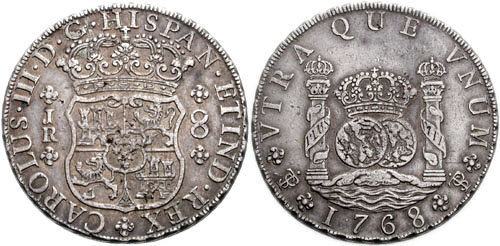
\includegraphics[width=0.38\textwidth]{coin}}

\begin{itemize}
\item You are presented with a coin: what is the probability of heads?\\
\hfill\Blue{\emph{What does this question even mean?}}

\item How much are you willing to bet $p({\rm head})>0.5$?\\
\hfill\Red{\emph{Do you expect this coin to come up heads more often that tails?}}\\
\hfill\Blue{\emph{Wait... can you toss the coin a few times, I need data!}}

\item Ok, you observe the following sequence of outcomes ($T$: tail, $H$: head):\\
\centerline{$H$}
\hfill\Blue{\emph{This is not enough data!}}

\item Now you observe the outcome of three additional tosses:\\
\centerline{$H HTH$}
How much are you \Red{\emph{now}} willing to bet $p({\rm head})>0.5$?
\end{itemize}

\end{frame}

\begin{frame}
\frametitle{The Bernoulli discrete binary distribution}

The \Blue{\emph{Bernoulli}} probability distribution over binary random variables:
\begin{itemize}
\item Binary random variable $X$: outcome $x$ of a single coin toss.
\item The two values $x$ can take are
\begin{itemize} 
\item $X=0$ for tail,
\item $X=1$ for heads.
\end{itemize}
\item Let the probability of heads be $\pi=p(X=1)$.\\
$\pi$ is the \Blue{\emph{parameter}} of the Bernoulli distribution.
\item The probability of tail is $p(X=0)=1-\pi$. We can compactly write
  \begin{equation*}
    p(X=x|\pi)\;=\;p(x|\pi)\;=\;\pi^x (1-\pi)^{1-x}
  \end{equation*}
\end{itemize}

What do we think $\pi$ is after observing a single heads outcome?
\begin{itemize}
\item Maximum likelihood! Maximise $p(H|\pi)$ with respect to\ $\pi$:
\[
p(H|\pi)\;=\;p(x=1|\pi)\;=\;\pi\,,
{\; \; \; \; \; \; }
\argmax_{\pi\in[0,1]} \pi = 1
\]
\item Ok, so the answer is $\pi=1$. This coin only generates heads.\\
\hfill\Red{\emph{Is this reasonable? How much are you willing to bet p(heads)>0.5?}}\\
\end{itemize}

\end{frame}


\begin{frame}
\frametitle{The binomial distribution: counts of binary outcomes}

We observe a sequence of tosses rather than a single toss:
\centerline{$HHTH$}

\begin{itemize}
\item The probability of this particular sequence is:\; $p(HHTH)=\pi^3(1-\pi)$.
\item But so is the probability of $THHH$, of $HTHH$ and of $HHHT$.
\item We often don't care about the order of the outcomes, only about the \Blue{\emph{counts}}.\\
In our example the probability of 3 heads out of 4 tosses is:\; $4\pi^3(1-\pi)$.
\end{itemize}

The \Blue{\emph{binomial distribution}} gives the probability of
observing $k$ heads out of $n$ tosses
\[
p(k|\pi,n)\;=\; 
\big(\!\!\begin{array}{c}n\\k\end{array}\!\!\big)\pi^k(1-\pi)^{n-k}
\]
\begin{itemize}
\item This assumes $n$ independent tosses from a Bernoulli distribution $p(x|\pi)$.
\item $\big(\!\!\begin{array}{c}n\\k\end{array}\!\!\big)=\frac{n!}{k!(n-k)!}$ is the 
binomial coefficient, also known as ``n choose k''.
\end{itemize}

\end{frame}

\begin{frame}
\frametitle{Naming of discrete distributions}

\begin{center}
\begin{tabular}{|l|l|l|}
\hline
& binary & multi-valued\\ \hline
sequence & binary categorical $\pi^k(1-\pi)^{n-k}$ & categorical $\prod_{i=1}^k\pi_i^{k_i}$ \\ \hline
counts & binomial
         $\big(\!\!\begin{array}{c}n\\k\end{array}\!\!\big)\pi^k(1-\pi)^{n-k}$
& multinomial \frac{n!}{_1!k_2!\ldots k_m!}\prod_{i=1} \pi_i^{k_i}\\ \hline
\end{tabular}
\end{center}

For binary outcomes with have $k$ successes in $n$ trials. For
multi-dimensional distributions we have $k$ possible outcomes, a
sequence $x_1,\ldots,x_N$ and counts $c_i=\sum_{n=1}^N\delta(x_n,i)$
. For all distributions the parameter of the distribution is the
vector ${\boldsymbol\pi}$, which has either one element
$\pi \in [0; 1]$ or multiple entries such that $\pi_i>0$ and
$\sum_i\pi_i=1$.



\end{frame}


\begin{frame}
\frametitle{Maximum likelihood under a binomial distribution}

If we observe $k$ heads out of $n$ tosses, what do we think $\pi$ is?

We can maximise the likelihood of parameter $\pi$ given the observed data.
\[
p(k|\pi,n)\;\propto\;\pi^k(1-\pi)^{n-k}
\]
It is convenient to take the logarithm and derivatives with respect to $\pi$
\begin{align*}
\log p(k|\pi,n)\;&=\;k\log\pi + (n-k)\log(1-\pi) + \mathrm{Constant}\\
\frac{\partial \log p(k|\pi,n)}{\partial \pi}\;&=\; \frac{k}{\pi} - \frac{n-k}{1-\pi}
=0\;\iff\;\boxed{\pi\;=\;\frac{k}{n}}
\end{align*}

Is this reasonable? 
\begin{itemize}
\item For $HHTH$ we get $\pi=3/4$. 
\item How much would you bet now that $p({\rm heads})>0.5?$\\
\hfill\Red{\emph{What do you think $p(\pi>0.5) is$?}}\\
\hfill\Blue{\emph{Wait! This is a probability over ... a probability?}}
\end{itemize}

\end{frame}


\begin{frame}
\frametitle{Prior beliefs about coins -- before tossing the coin}

So you have observed 3 heads out of 4 tosses but are unwilling to bet
£100 that $p(heads)>0.5$?

\hfill (That for example out of 10,000,000 tosses at least 5,000,001 will be heads)

\hspace{1ex}

Why?

\begin{itemize}
\item You might believe that coins tend to be fair ($\pi\simeq\tfrac{1}{2}$).
\item A finite set of observations \Blue{\emph{updates your opinion}} about $\pi$.
\item But how to express your opinion about $\pi$ \Blue{\emph{before}} you see any data?
\end{itemize}
\Blue{\emph{Pseudo-counts}}: You think the coin is fair and... you are...
\begin{itemize}
\item Not very sure. You act as if you had seen 2 heads and 2 tails before.
\item Pretty sure. It is as if you had observed 20 heads and 20 tails before.
\item Totally sure. As if you had seen 1000 heads and 1000 tails before.
\end{itemize}

Depending on the strength of your prior assumptions, it takes a
different number of actual observations to change your mind.


\end{frame}
\begin{frame}
\frametitle{The Beta distribution: distributions on \emph{probabilities}}

Continuous probability distribution defined on the interval
$[0,1]$
\[
\mathrm{Beta}(\pi|\alpha,\beta)\;=\;
\frac{\Gamma(\alpha+\beta)}{\Gamma(\alpha)\Gamma(\beta)}
\pi^{\alpha-1}(1-\pi)^{\beta-1}
\;=\;\frac{1}{B(\alpha,\beta)}\pi^{\alpha-1}(1-\pi)^{\beta-1}
\]
\vspace{-4mm}
\begin{itemize}
\item $\alpha>0$ and $\beta>0$ are the shape \Blue{\emph{parameters}}.
\item these parameters correspond to `one plus the pseudo-counts'.  
\item $\Gamma(\alpha)$ is an extension of the factorial function\footnote{$\Gamma(\alpha)
  =\int_0^\infty x^{\alpha-1} e^{-x} dx$}. 
$\Gamma(n)=(n-1)!$ for integer $n$.
\item $B(\alpha,\beta)$ is the beta function, it normalises the Beta distribution.
\item The mean is given by $E(\pi)=\frac{\alpha}{\alpha+\beta}$.\hfill
[Left: $\alpha=\beta=1$, Right:  $\alpha=\beta=3$]
\end{itemize}

\centerline{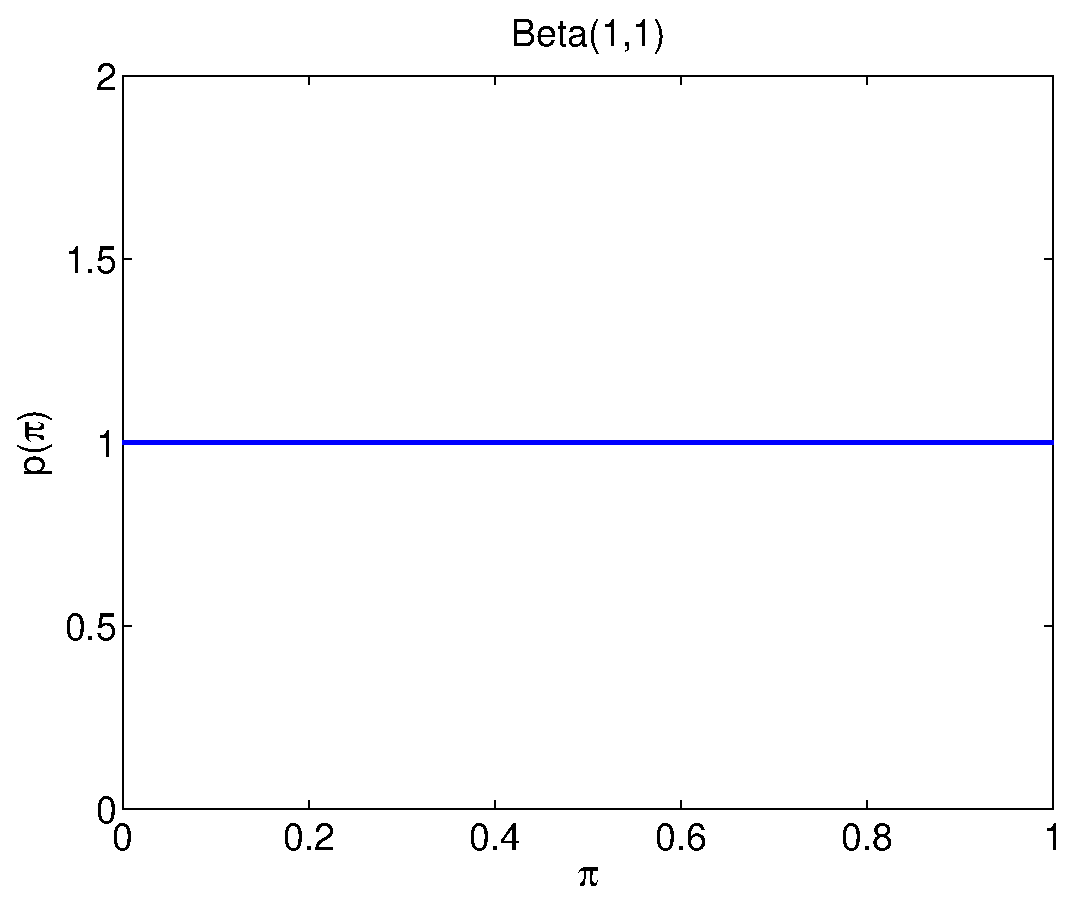
\includegraphics[width=0.3\textwidth]{Beta11}
\hspace{1cm}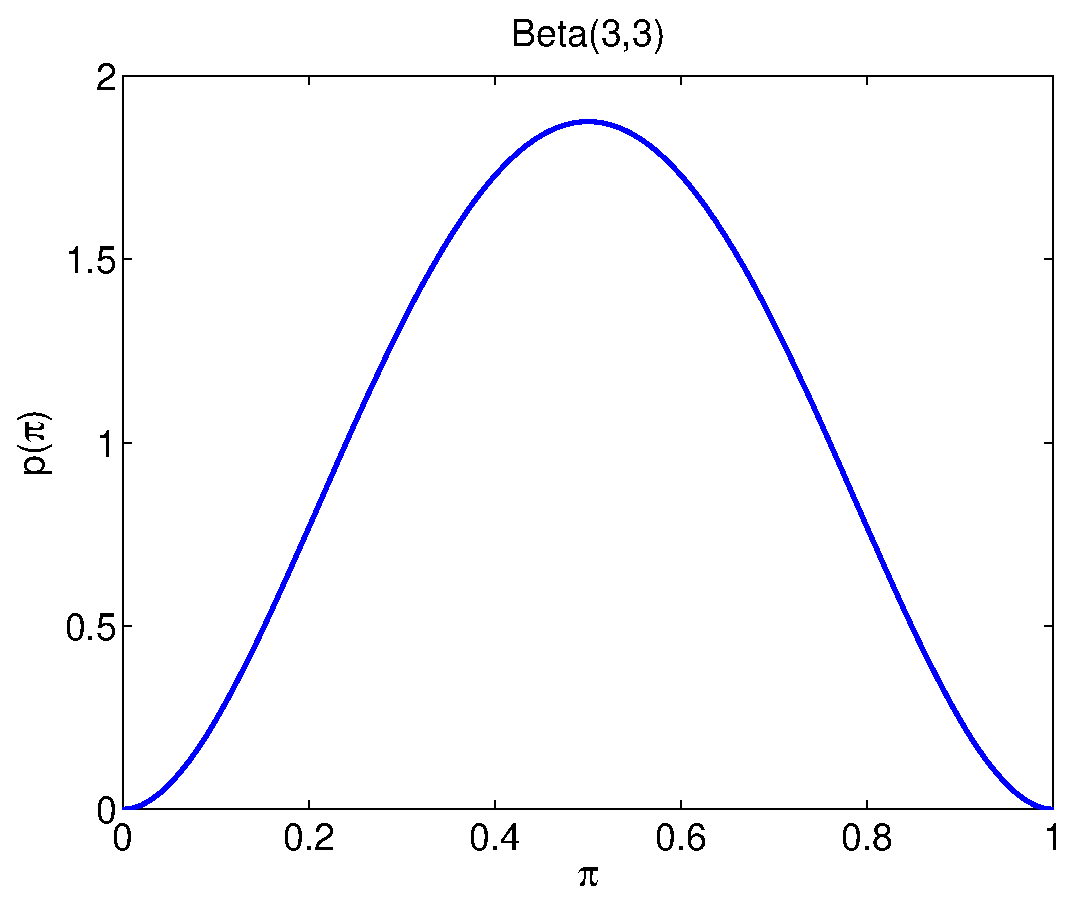
\includegraphics[width=0.3\textwidth]{Beta33}}
\end{frame}


\begin{frame}
\frametitle{Posterior for coin tossing}

Imagine we observe a single coin toss and it comes out heads. Our observed data is:
\[
\mathcal{D}\;=\;\{k=1\},\text{\ \ \ \ where\ \ \ \ }n=1.
\]

The probability of the observed data given $\pi$ is the \Blue{\emph{likelihood}}:
\[
\Blue{p(\mathcal{D}|\pi)}\;=\;\pi
\]

We use our \Red{\emph{prior}} \Red{$p(\pi|\alpha,\beta)=\mathrm{Beta}(\pi|\alpha,\beta)$}  
to get the \PineGreen{\emph{posterior}} probability:
\begin{eqnarray*}
\PineGreen{p(\pi|\mathcal{D})}&=&\frac{\Red{p(\pi|\alpha,\beta)}
\Blue{p(\mathcal{D}|\pi)}}{p(\mathcal{D})}\;\propto\;\pi \; \mathrm{Beta} (\pi|\alpha,\beta) \\[2ex]
& \propto& \pi \; \pi^{(\alpha-1)} (1-\pi)^{(\beta-1)} 
\;\propto\;\PineGreen{\mathrm{Beta}(\pi|\alpha+1,\beta)}
\end{eqnarray*}

The Beta distribution is a \Blue{\emph{conjugate}} prior to the
Bernoulli/binomial distribution:
\begin{itemize}
\item The resulting posterior is also a Beta distribution.
\item The posterior parameters are given by: 
$\begin{array}{l}\alpha_{\rm posterior}=\alpha_{\rm prior}+k\\ 
\beta_{\rm posterior}=\beta_{\rm prior}+(n-k)\end{array}$
\end{itemize}

\end{frame}


\begin{frame}
\frametitle{Before and after observing one head}

\centerline{Prior}

\centerline{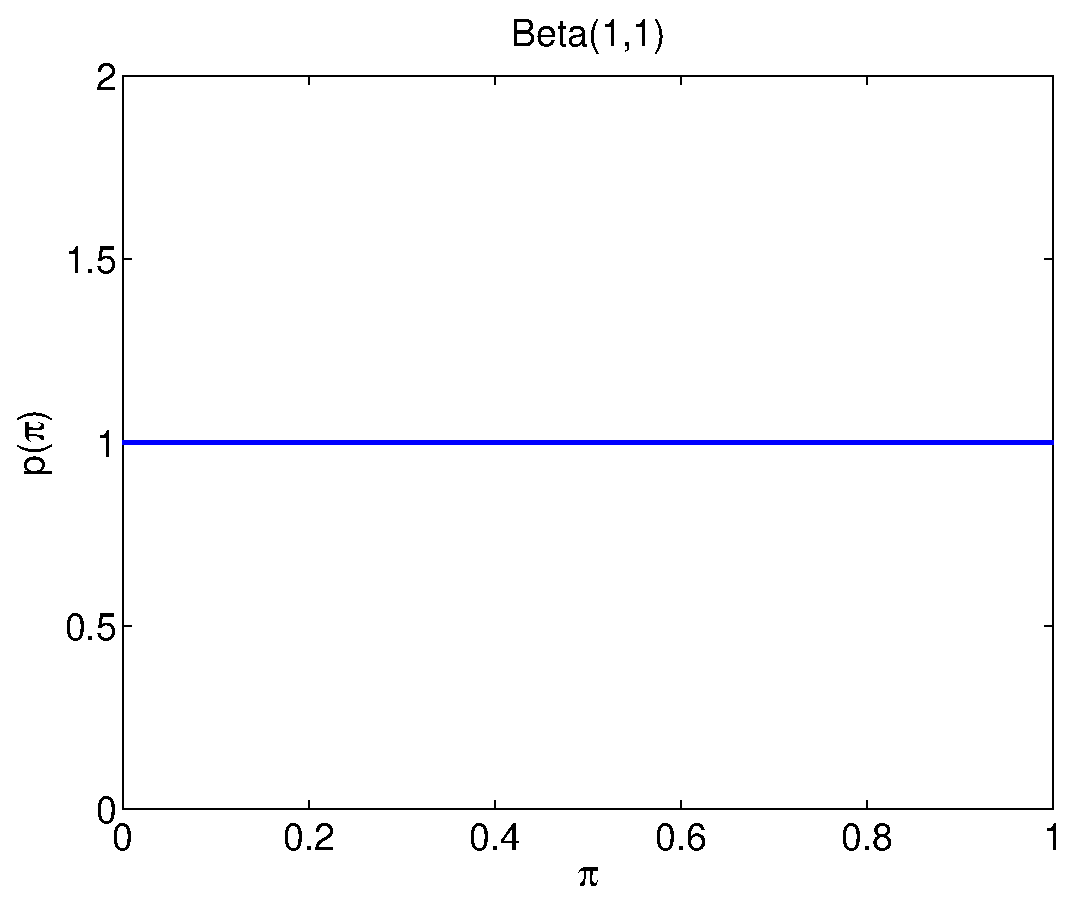
\includegraphics[width=0.3\textwidth]{Beta11}\hspace{2cm}
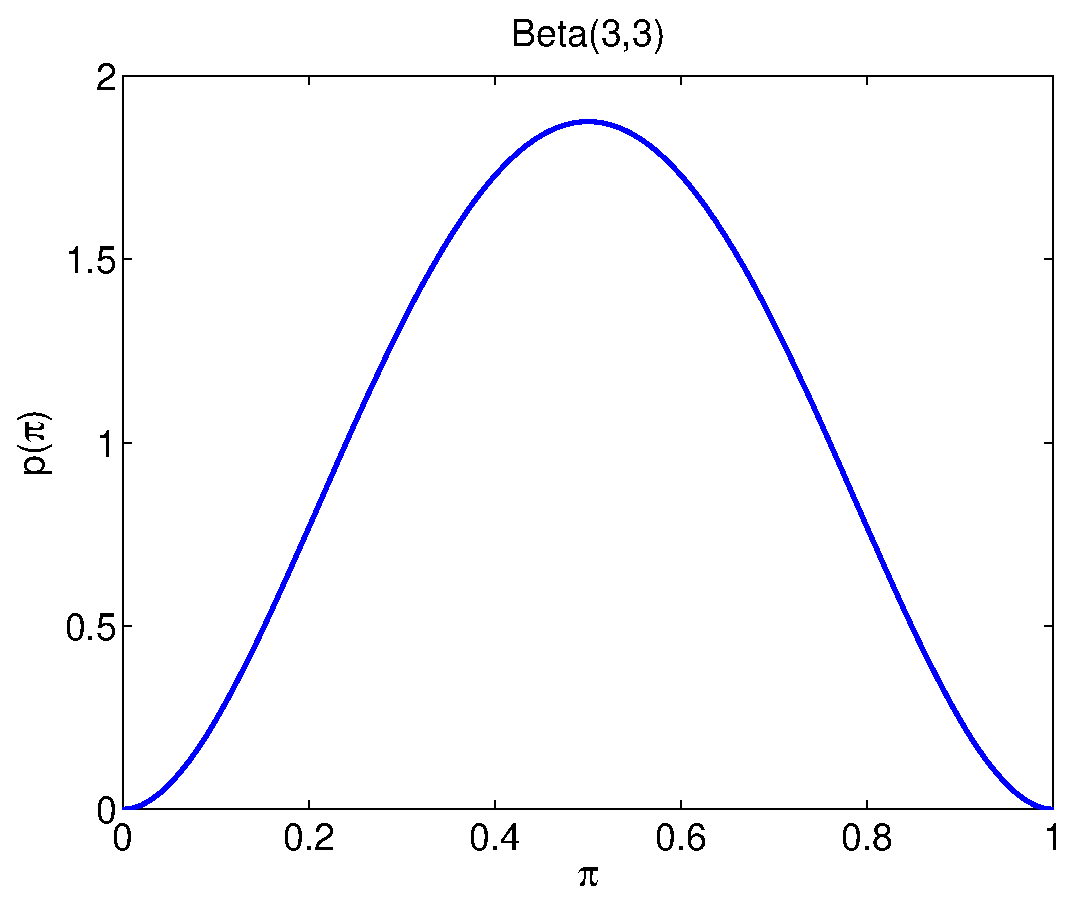
\includegraphics[width=0.3\textwidth]{Beta33}}


\centerline{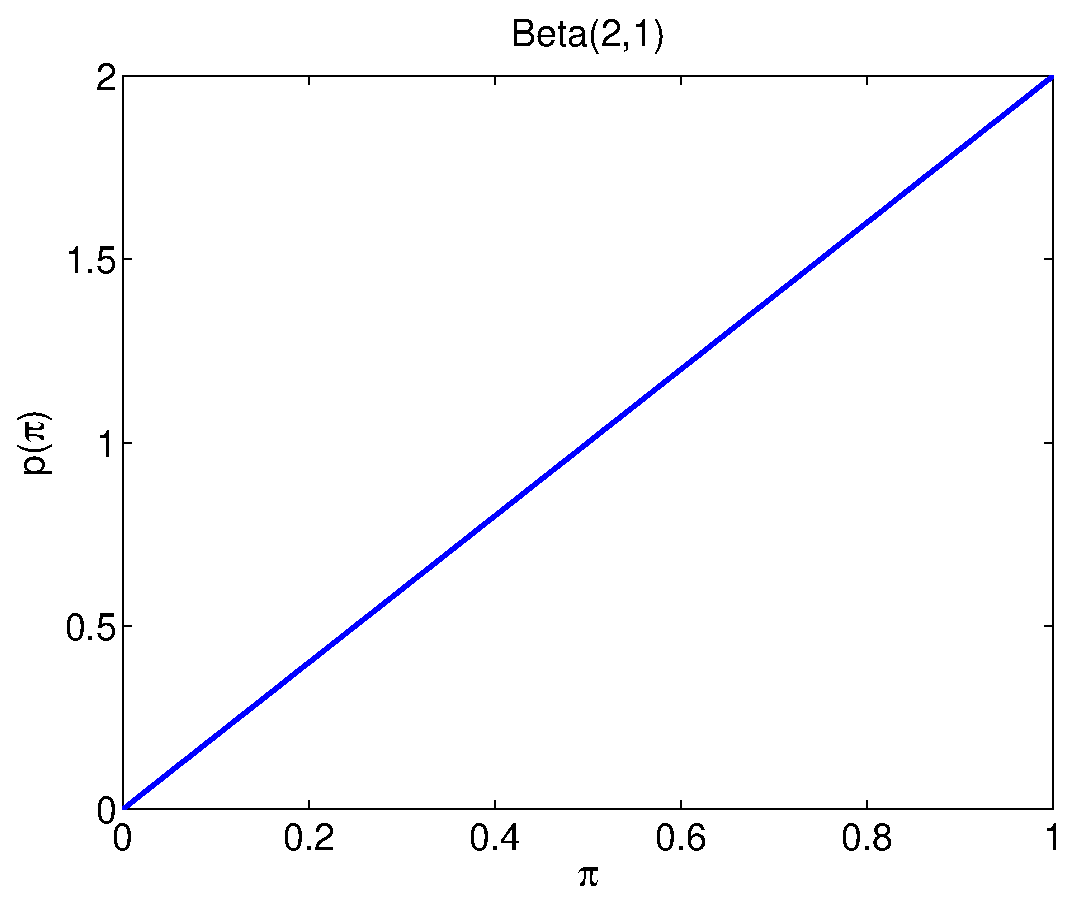
\includegraphics[width=0.3\textwidth]{Beta21}\hspace{2cm}
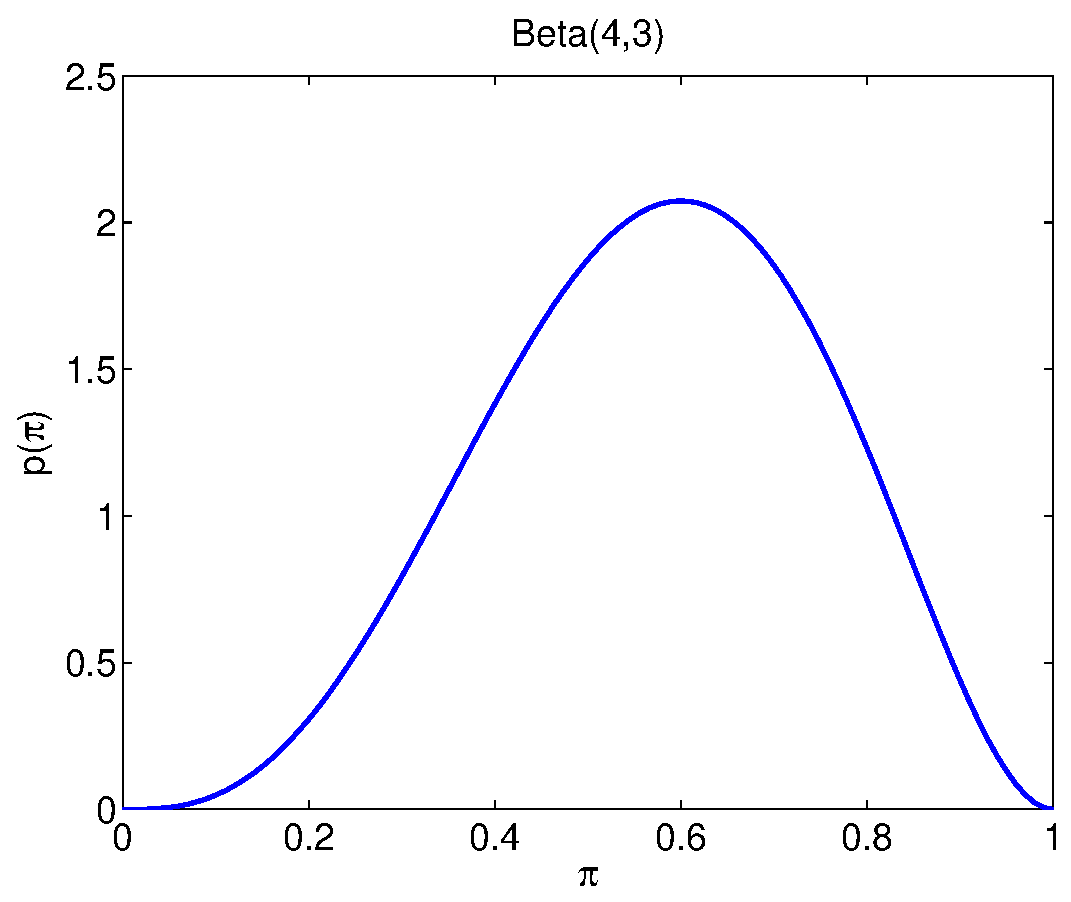
\includegraphics[width=0.3\textwidth]{Beta43}}

\centerline{Posterior}
\end{frame}

\begin{frame}
\frametitle{Making predictions}

Given some data $\cal D$, what is the predicted probability of the
next toss being heads, $x_{\mathrm{next}}=1$?

Under the Maximum Likelihood approach we predict using the value of
$\pi_{\mathrm{ML}}$ that maximises the likelihood of $\pi$ given the observed data, ${\cal D}$:
\[
p(x_{\mathrm{next}}=1|\pi_{\mathrm{ML}}) = \pi_{\mathrm{ML}}
\]

With the Bayesian approach, \Red{\textbf{average} over all
  possible parameter settings:}
%
\[
p(x_{\mathrm{next}}=1|{\cal D})\;=\;\int p(x=1|\pi)\,\PineGreen{p(\pi|{\cal D})}\,{\rm d}\pi
\]
%
The prediction for heads happens to correspond to
the mean of the \PineGreen{\emph{posterior}}
distribution. E.g.\ for  ${\cal D} = \{(x=1)\}$:
\begin{itemize}
\item \Red{Learner A with $\mathrm{Beta}(1,1)$} predicts $p(x_{\mathrm{next}}=1|{\cal D}) = \frac{2}{3}$
\item \Blue{Learner B with $\mathrm{Beta}(3,3)$} predicts
  $p(x_{\mathrm{next}}=1|{\cal D}) = \frac{4}{7}$ 
\end{itemize}
\end{frame}


\begin{frame}
\frametitle{Making predictions - other statistics}

Given the posterior distribution, we can also answer other questions
such as ``what is the probability that $\pi>0.5$ given the observed
data?''
%
\[
p(\pi>0.5|{\cal D}) 
\;=\;\int_{0.5}^1 p(\pi'|{\cal D})\,{\rm d}\pi'
\;=\;\int_{0.5}^1 \mathrm{Beta}(\pi'|\alpha', \beta'){\rm d}\pi'
\]
%

\begin{itemize}
\item \Red{Learner A with prior $\mathrm{Beta}(1,1)$} predicts $p(\pi>0.5|{\cal D}) = 0.75$
\item \Blue{Learner B with prior $\mathrm{Beta}(3,3)$} predicts $p(\pi>0.5|{\cal D}) = 0.66$
\end{itemize}

% Note that for any $\ell>1$ and fixed $\alpha$ and $\beta$, the two
% posteriors $\mathrm{Beta}(\pi|\alpha,\beta)$ and
% $\mathrm{Beta}(\pi|\ell\alpha,\ell\beta)$ have the
% same  \emph{average} $\pi$, but give different values for $p(\pi>0.5)$.

\end{frame}


\begin{frame}
\frametitle{Learning about a coin, multiple models (1)}

Consider two alternative models of a coin, ``fair'' and ``bent''. A
priori, we may think that ``fair'' is more probable, eg:
%
\[
p({\rm fair})\;=\;0.8,\qquad p({\rm bent})\;=\;0.2
\]
For the bent coin, (a little unrealistically) all parameter values
could be equally likely, where the fair coin has a fixed probability: \\[2ex]

\centerline{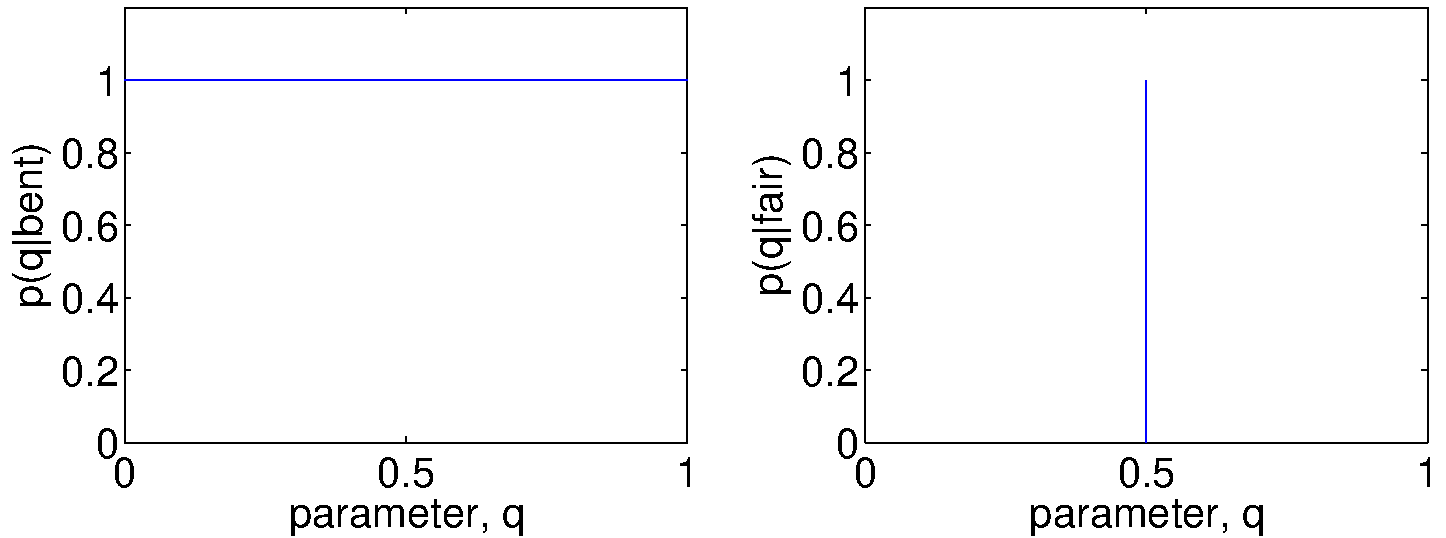
\includegraphics[width=0.7\textwidth]{Beta11andBetaInfInf}}

\end{frame}


\begin{frame}
\frametitle{Learning about a coin, multiple models (2)}

We make $10$ tosses, and get data ${\cal D}$: T H T H T T T T T T

The \Red{evidence} for the fair model is: $
p({\cal D}|{\rm fair}) = (1/2)^{10}\simeq 0.001
$\\
and for the bent  model:
\begin{equation*}
p({\cal D}|{\rm bent}) = \int p({\cal D}|\pi,{\rm bent})p(\pi|{\rm
  bent})  \; d\pi =  \int  \pi^2(1-\pi)^8 \; d\pi={\rm B}(3,9)\simeq 0.002
\end{equation*}

Using priors $p({\rm fair})=0.8$, $p({\rm bent})=0.2$, the posterior by Bayes rule:
\[
p({\rm fair}|{\cal D}) \propto 0.0008,\qquad p({\rm bent}|{\cal D}) \propto
0.0004,
\]
ie, two thirds probability that the coin is fair.

{\bf How do we make predictions?} By weighting the predictions from each
model by their probability. Probability of Head at next toss is:
\[
\frac{2}{3}\times \frac{1}{2} + \frac{1}{3}\times \frac{3}{12} = \frac{5}{12}.
\]
\end{frame}

\end{document}